\subsubsection{Entidades y atributos}

Las diferentes entidades junto con sus atributos son las siguientes: \textcolor{red}{mirar la definición de cada uno de los atributos de las entidades, además de mirar bien las relaciones}
\begin{itemize}
    \item \textbf{Pigmento}: tenemos que almacenar de una manera segura y persistente la información relacionada con cada uno de los pigmentos. Para ello simplemente vamos a exportar dichos datos de las bases de datos ya existentes y creadas en AccessDB. La información que tenemos que almacenar de cada uno de los pigmentos es la siguiente:
        \begin{itemize}
            \item \textit{Nombre}: nombre con el que se identifica a cada uno de los pigmentos dentro de la base de datos. Dicho nombre es único para cada uno de los pigmentos.
            \item \textit{Id Color}: id representando el color principal de cada uno de los pigmentos
            \item \textit{Notas}: los pigmentos pueden o no tener notas adjuntas, de hecho se permite a los usuarios añadir notas sobre dichos pigmentos. Es por ello que se permiten almacenar notas separadas de cada uno de los elementos de la base de datos.
            \item \textit{Potencia}: \textcolor{red}{TODO}
            \item \textit{Lambda}: \textcolor{red}{TODO}
            \item \textit{Fórmula}: los pigmentos al estar compuestos por elementos naturales, tienen fórmulas químicas determinadas. Es un dato importante si queremos saber su composición o como van a reaccionar cuando están en presencia de cierto elementos químicos, también la mostraremos.
            \item \textit{Sinónimos}: los pigmentos pueden tener sinónimos a la hora de ser llamados. Es por esto que cada uno de ellos tendrá una relación con sus sinónimos. 
            \item \textit{Elemento químico}: cada uno de los pigmentos tiene un elemento químico predominante en su composición química. Tenemos que almacenarlo para mostrarlo cuando proporcionemos la información relacionada con el pigmento.
        \end{itemize}
        
    \item \textbf{Colorimetría}:
        \begin{itemize}
            \item \textit{L}: \textcolor{red}{TODO}
            \item \textit{a}: \textcolor{red}{TODO}
            \item \textit{b}: \textcolor{red}{TODO}
            \item \textit{X}: \textcolor{red}{TODO}
            \item \textit{Y}: \textcolor{red}{TODO}
            \item \textit{Z}: \textcolor{red}{TODO}
            \item \textit{\textcolor{red}{TODO}}: \textcolor{red}{TODO}
        \end{itemize}
        
    \item \textbf{Difractograma de rayos X}:
        \begin{itemize}
            \item \textit{x}: \textcolor{red}{TODO}
            \item \textit{y}: \textcolor{red}{TODO}
        \end{itemize}
        
    \item \textbf{Espectro de Raman}:
        \begin{itemize}
            \item \textit{x}: \textcolor{red}{TODO}
            \item \textit{y}: \textcolor{red}{TODO}
        \end{itemize}
        
    \item \textbf{Espectro de infrarrojos}:
        \begin{itemize}
            \item \textit{x}: \textcolor{red}{TODO}
            \item \textit{y}: \textcolor{red}{TODO}
        \end{itemize}
        
    \item \textbf{Notas}: el usuario tiene que ser capaz de escribir notas rápidas para sí mismo acerca de cada uno de los pigmentos. Es por ello que una de las opciones de la aplicación es almacenar notas de uno de los pigmentos seleccionados. Dichas notas podrán ser recuperadas con posterioridad por el usuario para ser editadas o borradas.
        \begin{itemize}
            \item \textit{Título}: cada una de las notas que almacenamos de un pigmento consta de un título, que no es único y va a tener una longitud limitada a 100 caracteres. Tiene que ser algo corto y determinado. Ya que lo primero que ser verá cuando mostremos la vista de las notas es el título y estarán ordenadas por la fecha de creación, por lo que la última nota creada es la que se mostrará por completo. 
            \item \textit{Valor}: el valor es la nota en sí. Lo que el usuario introduzca en el formulario de escritura. 
            \item \textit{Fecha}: la fecha no será necesario mostrarla al usuario, pero si que tiene sentido almacenarla en la base da datos para tener un histórico de creación de las mismas y luego poder recuperarlas en diferente orden por la aplicación.  
        \end{itemize}
        
    \item \textbf{Sinónimos}: cada uno de los pigmentos puede tener nombres diferentes con los que ha sido referenciado a lo largo del tiempo. Es por esto que tendremos un lista para cada uno de los pigmentos con todos los sinónimos que tenga. 
        \begin{itemize}
            \item \textit{Valor}: como cada uno de los sinónimos puede tener 0 o más sinónimos, he decidido hacer una relación separada para cada uno de los pigmentos. Sino otra forma es hacer un atributo sinónimo dentro de la entidad Pigmento conteniendo una lista separada por comas con todos los sinónimos, pero me parece una mejor opción hacer una relación separada. 
        \end{itemize}
\end{itemize}

Antes de mostrar el diagrama de entidad relación vamos a mostrar una pequeña tabla con las diferentes cardinalidades y entidades relacionadas. Podemos encontrar dicho gráfico en la \textbf{Figura \ref{fig:cardinalidades}}

\begin{figure}[H]
    \centering
    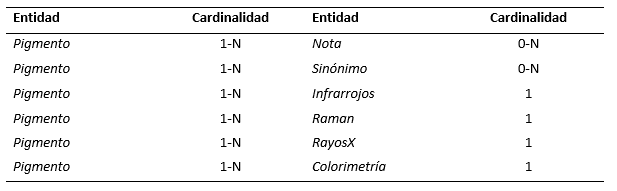
\includegraphics[scale=1]{imagenes/disenoBaseDatos/cardinalidades.png}
    \caption{Entidades y cardinalidades del modelo}
    \label{fig:cardinalidades}
\end{figure}

\subsubsection{Diagrama de Entidad Relación}

Una vez que hemos presentado tanto las entidades, como las cardinalidades y como están relacionadas las mismas, podemos mostrar como se relacionan las unas con las otras de una manera gráfica, que es presentado el diagrama de entidad relación de la base de datos. En este caso se ha decidido usar el formato de UML y no sigue las reglas estrictas del modelo de Entidad Relación, pero me parece que es más visual, la herramienta y el formato es más universal y entendible que el propio para expresar este tipo de contenidos. Podemos encontrar esto en la \textbf{Figura \ref{fig:diagramaER}}

\begin{figure}[H]
    \centering
    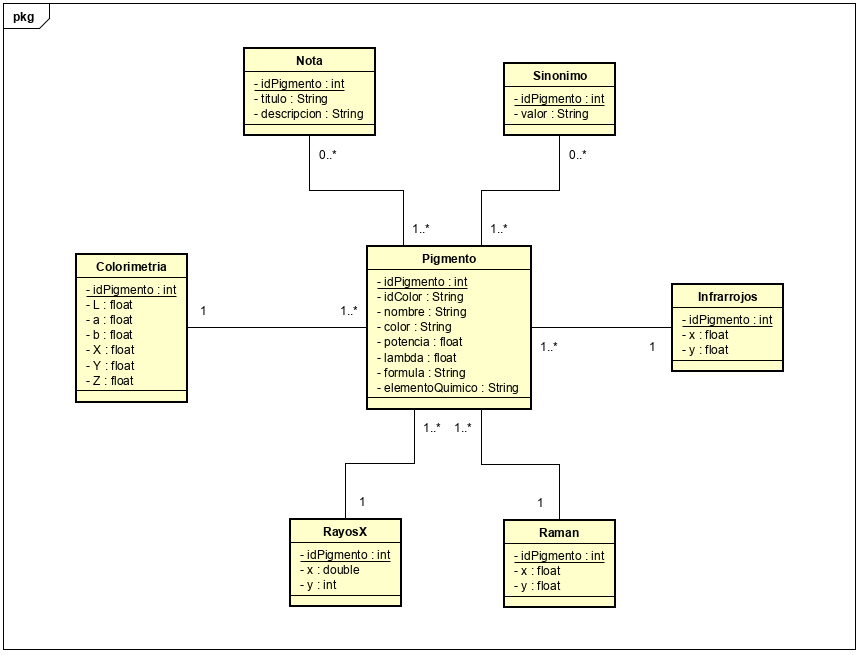
\includegraphics[scale=0.75]{imagenes/disenoBaseDatos/diagramaER.png}
    \caption{Diagrama de Entidad-Relación de la base de datos}
    \label{fig:diagramaER}
\end{figure}

En el diagrama podemos observar como la clave primaria de todas las relaciones es el id del pigmento en cuestión. Esto luego nos permitirá conectar unas relaciones con otras y buscar la información de una manera más adecuada. 

\textcolor{red}{mirar a ver las transformaciones y buscar un poco mas de teoría de diseño de la base de datos}

Una vez que tenemos el diseño de la base de datos podemos pasar a explicar la implementación de la misma, en lineas generales. 
